Over the last 20 years, the Internet of Things has developed and evolved continuously, from 20 years ago where it was the concept of using barcodes, and later RFID\cite{K.Ashton}, to track items in a warehouse, to today where our home appliances are filled with ``smart'' electronics, able to sense, react and notify the user of events, such as the washing machine finishing a load. Whilst the Internet of Things has been around for quite some time, under various guises, it's yet to become commercially successful and see wide-spread deployment; Many believe that 2013 is the year that the Internet of Things will truly take off and become ubiquitous in our daily lives\cite{2013IoT}.

The rest of this section will discuss the various different attempts made to create Internet of Things networks in the home.

\subsubsection{Smart Things} % (fold)
\label{ssub:smart_things}
Launched in 2012, the SmartThings platform aims to allow the user to turn any ordinary object in the home into a ``Smart'' object by giving it the ability to connect to the Internet. The platform consists of a central hub connected to the Internet, containing a low-power Zigbee radio, from which it connects to an array of SmartThings accessories as well as many pre-existing third party Zigbee devices. Some of these accessories include motion detectors, moisture sensors, vibration detectors, power-plug switches as well as many others. The user can then view and interact with their Smart Things through the cloud service via an Internet-connected PC or a smartphone, allowing them to either control the devices directly or set-up rules/schedules for devices.

\begin{figure}[h!]
\centering
    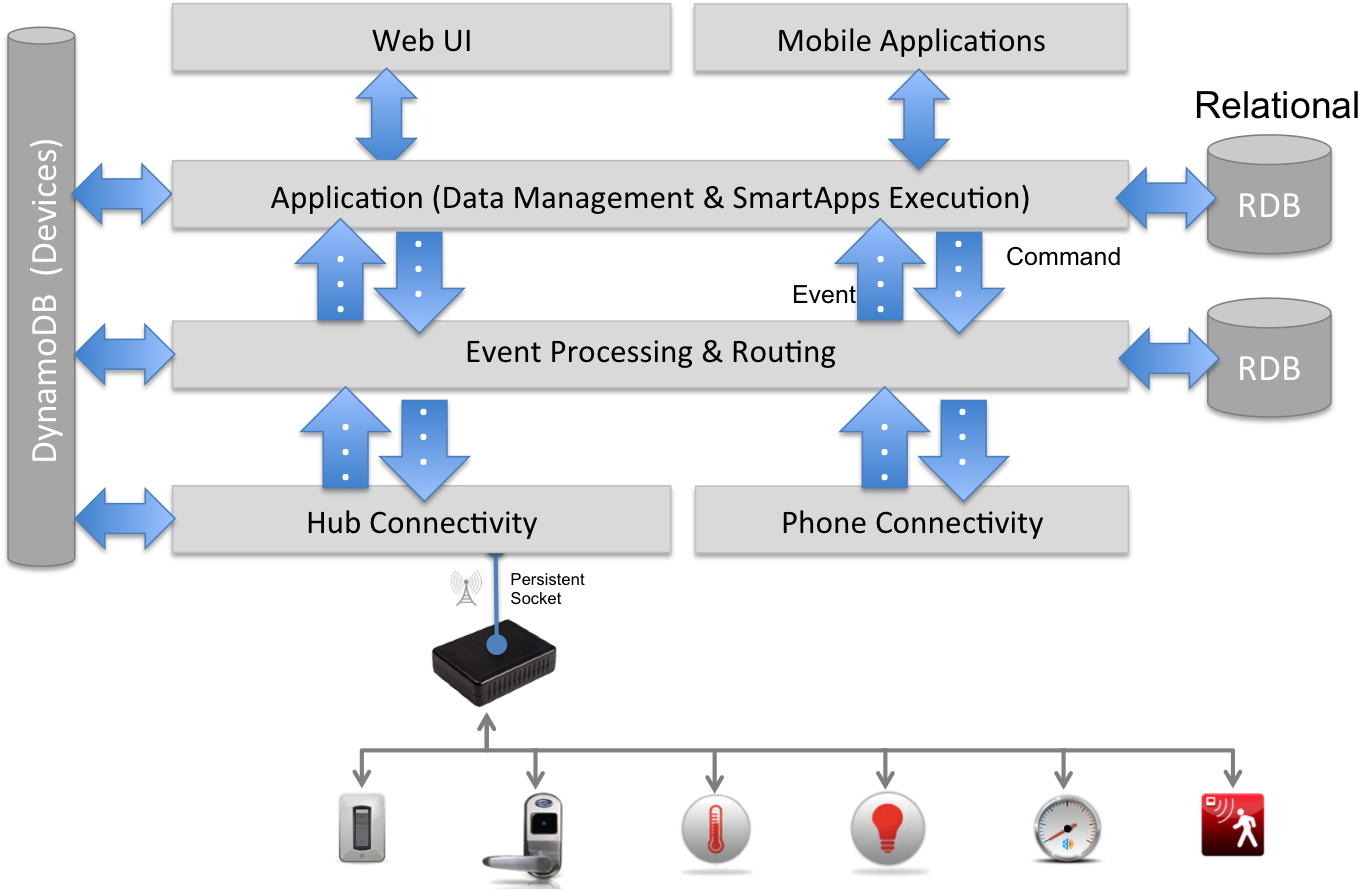
\includegraphics[scale=0.4]{images/smartThingsCloudFirstDiagram.png}
    \caption[]{Smart Things - Cloud approach\footnotemark}
    \label{fig:cloud}
\end{figure}
\footnotetext{Image from Smart Things developer support: \url{https://support.smartthings.com/entries/21603009-Device-Types-Capabilities-Attributes}}

As shown in figure \ref{fig:cloud}, Smart Things takes a cloud approach, offloading all processing to the cloud, leaving the hub to just act as a gateway and translator between the Things and the cloud. By utilising the cloud in this way, it enables the hub to be a very simple and low-power device, reducing the costs for the user. It also allows the user to access their network of Things from anywhere, at any time, which would otherwise be difficult to do in a local approach. 

However, the cloud approach also has several drawbacks. By offloading the entire processing needs of the network, as show above, the network of Things becomes vulnerable to failure if either the network fails or is unresponsive, or if the cloud service fails or goes down for maintenance. Another issue is the privacy of the user's data; How safe is the data in the cloud and how secure are the services they make available for users to interact with their devices with. There have been many examples of online services that have been attacked, leaking user data and/or shutting down for extended periods of time \cite{Playstation, Amazon, Google}.

Talk about integration of two home networks.


% Currently, there is no information on how the underlying protocol for connecting the SmartThings to the hub works, but at the time of writing, the current implementation uses a ``cloud first'' approach. This means that rather than the hub wiring all devices together based on the rules and schedules set up by the user, all the intelligence of the network is being handled in the cloud. This brings about the problem of Internet connectivity, with two points of failure, either the user or the cloud. From the user's standpoint, an Internet connection might not be available where the hub is located, or the user could have a faulty, slow or non-permanent connection, which renders all the SmartThings devices into dumb devices. In contrast to this, because of the reliance on the cloud, if the cloud service provider experiences downtime then all SmartThings users devices become dumb devices. In cases where these devices are used for security and safety, dire consequences could result.
% subsubsection smart_things (end)

\subsubsection{CoRE CoAP} % (fold)
\label{ssub:core_coap}

% subsubsection core_coap (end)
\subsubsection{KNoT} % (fold)
\label{ssub:knot}

% subsubsection knot (end)